
\RequirePackage{plautopatch}  % pLaTeX または upLaTeX のとき
%\documentclass[uplatex,dvipdfmx,titlepage,a4j]{jsarticle}% upLaTeX のとき
\documentclass[dvipdfmx,titlepage,a4j]{jsarticle}  % pLaTeX のとき
\usepackage{listings,jvlisting}
\usepackage{amsmath,amssymb}
\usepackage{graphicx}
\usepackage[yen]{okuverb}
\usepackage{r04ec-exp}
\usepackage{here}
\usepackage{ascmac}
\usepackage{fancybox}
\usepackage{fancyvrb}
\usepackage{fancyhdr}
\usepackage{lastpage}
\usepackage{cases}
\usepackage[hang,small,bf]{caption}
\usepackage[subrefformat=parens]{subcaption}

\fancypagestyle{foot}
{
\fancyhead[C]{OPアンプの基礎・応用}
\fancyfoot[C]{\thepage / \pageref{LastPage}}
\renewcommand\headrulewidth{0.4pt}
}

%ここからソースコードの表示に関する設定
\lstset{
  language={C++},
  basicstyle={\ttfamily},
  identifierstyle={\small},
  commentstyle={\smallitshape},
  keywordstyle={\small\bfseries},
  ndkeywordstyle={\small},
  stringstyle={\small\ttfamily},
  frame={tb},
  tabsize={2},
  breaklines=true,
  columns=[l]{fullflexible},
  numbers=left,
  xrightmargin=0zw,
  xleftmargin=3zw,
  numberstyle={\scriptsize},
  stepnumber=1,
  numbersep=1zw,
  lineskip=-0.5ex
}

\renewcommand{\lstlistingname}{リスト}
%ここまでソースコードの表示に関する設定

\title{OPアンプの基礎・応用}
% 学年・番号
\grade{4年42番}%
% 氏名
\author{鷲尾 優作}
% 班(後期は班に分かれて実験をする.そのときは,ここに班番号を記入する.)
\team{}
% 提出日
\date{2022年12月22日}
% 実験日
\expdate{2022年11月24日,12月1日,12月8日}
% 共同実験者
% グループに分かれて実験をするテーマでは,グループメンバーの番号名前を書く.
\coauthor{
  39番 & 宮崎 来\\
  40番 & 吉田 \\
  43番 & 渡辺 あかり\\
}
%
%記載例:
%\coauthor{%
%  2番 & 新潟 花子\\
%  11番 & 三条 次郎}
%%

\begin{document}
\pagestyle{foot}

\maketitle

\section{目的}
本実験では,OPアンプを用いた増幅回路・演算回路の特性を測定し,理解することを目的とする.

\section{OPアンプによる負帰還増幅}
OPアンプ(Operational Amplifier)は,負帰還によって入力電圧の増幅や演算を行うための素子である.
負帰還増幅についての理解を深めるため,技術的背景・歴史について述べる.

\paragraph{負帰還増幅理論の形成\\}
一般的にアンプは,内部に使用される真空管(現代ではトランジスタ)周波数に対して非線形な特性を示すため,非線形な増幅となる.
したがって中長距離の電気通信ネットワークなど回路内で何十回も増幅を行う場合,ノイズや歪みによって伝送信号が劣化してしまう.
デジタル通信が発展する前の電気通信では,この問題は致命的であった.

オペアンプは,この問題が顕著に現れる1900年代前半のアメリカ大陸横断通信線の建設過程に開発された.

1927年,アメリカ ベル研究所のハロルド・スティーブン・ブラックがゲインを犠牲にし増幅後の電圧を帰還させ比較しながら増幅することで
増幅の線形性を高める着想をして以来,第二次世界大戦中の火器管制ネットワークの設計過程等を得てOPアンプの基礎技術が形成されることとなる.

OPアンプは外部に接続する負帰還・入力素子を設計者が適切に選定することで線型な増幅を得られるよう設計されており,
OPアンプを安定して使用する方法が負帰還と勘違いされがちであるが,歴史的には逆のようである.

この研究はハリー・ナイキストやヘンドリック・ボードの研究成果と合わせて制御工学などの他分野へと展開していくこととなる.

\paragraph{ICオペアンプの誕生\\}
テキサスインスツルメンツ社とアメリカ陸軍通信部隊との電子回路小型化のニーズによって1959年,半導体チップに全ての回路を詰め込むIC技術が発明されると
さまざまな電気素子にIC化による小型化,高機能化が図られることとなった.OPアンプも例外ではなく,IC設計基礎技術の発展を得て1963年,フェアチャイルドセミコンダクター製$\mu$A702がICオペアンプとして初めて市場に提供された.
非対称電源特性やゲインの低さ等の問題を抱え市場に受け入れられなかったが,10年以上にわたるトランジスタの性能向上,内部構造の見直しによって
特性・使いやすさが向上し,現在のOPアンプの基礎技術が発展した.

\section{オペアンプによる演算}
OPアンプは以上のとおり,OPアンプは外部に接続する素子を設計者が適切に選定することで線型な演算増幅を可能とするICである.
R(抵抗)を用いる単純な増幅回路・反転増幅回路から,R(抵抗)C(キャパシタ)を組み合わせて設計する微分・積分回路,フィルタ回路,バッファ回路など
,さまざまな応用が存在する.

本実験では,反転増幅回路,微分・積分回路,バンドパスフィルタを扱う.

\paragraph{反転増幅回路\\}

\paragraph{微分回路\\}

\paragraph{積分回路\\}

\paragraph{バンドパスフィルタ\\}

\section{演算回路の特性測定}
反転増幅回路(case 1),微分回路(case 2.1),実用微分回路(case 2.2),積分回路(case 3.1),実用積分回路(case 3.2),バンドパスフィルタ(case 4)とし,
各回路の閉ループ利得,入力に対する出力の位相差を測定する.
\subsection{測定機器}
\begin{enumerate}
  \item ブレッドボード No.20
  \item 直流電源装置 TRACO POWER No.5
  \item 交流電源装置 KENWOOD AG-203 分類L151 帳1 番号99
  \item オシロスコープ GWINSTEK GDS-1022 No.19
\end{enumerate}

\subsection{case 1}
図\ref{fig:gr:case1}にcase 1の回路特性測定結果をグラフで示す.
\begin{figure}[H]
  \centering
  \begin{minipage}{8cm}
    \centering
    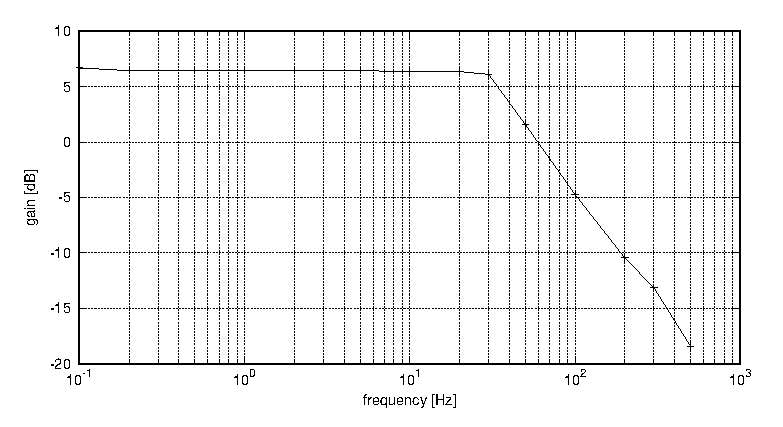
\includegraphics[keepaspectratio, scale=0.6]{../data/case1-g.eps}
    \subcaption{周波数対閉ループ利得特性}
  \end{minipage}
  \begin{minipage}{8cm}
    \centering
    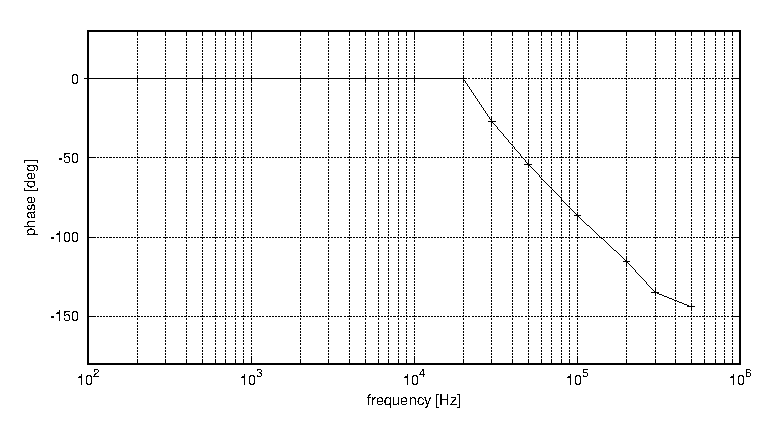
\includegraphics[keepaspectratio, scale=0.6]{../data/case1-f.eps}
    \subcaption{周波数対位相差特性}
  \end{minipage}
  \caption{case 1における回路特性測定結果}
  \label{fig:gr:case1}
\end{figure}

\subsection{case 2}
図\ref{fig:gr:case2}にcase 2.1 2.2の回路特性測定結果をグラフで重ねて示す.
\begin{figure}[H]
  \centering
  \begin{minipage}{8cm}
    \centering
    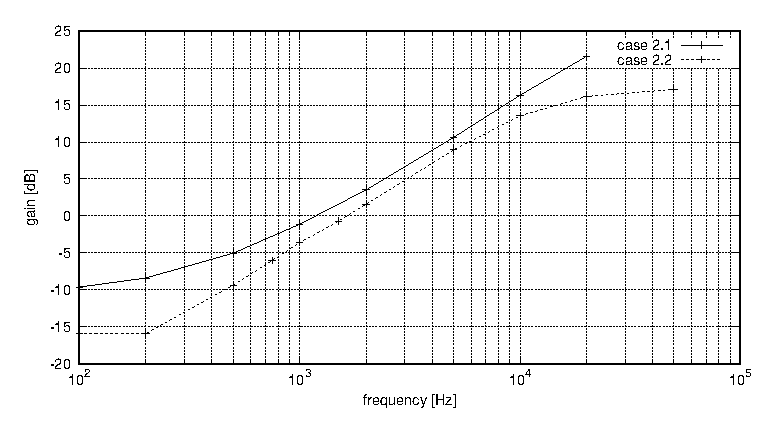
\includegraphics[keepaspectratio, scale=0.6]{../data/case2-g.eps}
    \subcaption{周波数対閉ループ利得特性}
  \end{minipage}
  \begin{minipage}{8cm}
    \centering
    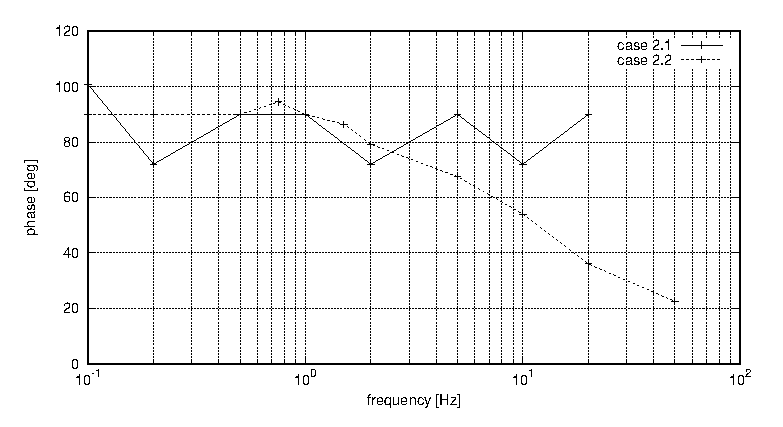
\includegraphics[keepaspectratio, scale=0.6]{../data/case2-f.eps}
    \subcaption{周波数対位相差特性}
  \end{minipage}
  \caption{case 2.1 2.2における回路特性測定結果}
  \label{fig:gr:case2}
\end{figure}

\subsection{case 3}
図\ref{fig:gr:case3}にcase 3.1 3.2の回路特性測定結果をグラフで重ねて示す.
\begin{figure}[H]
  \centering
  \begin{minipage}{8cm}
    \centering
    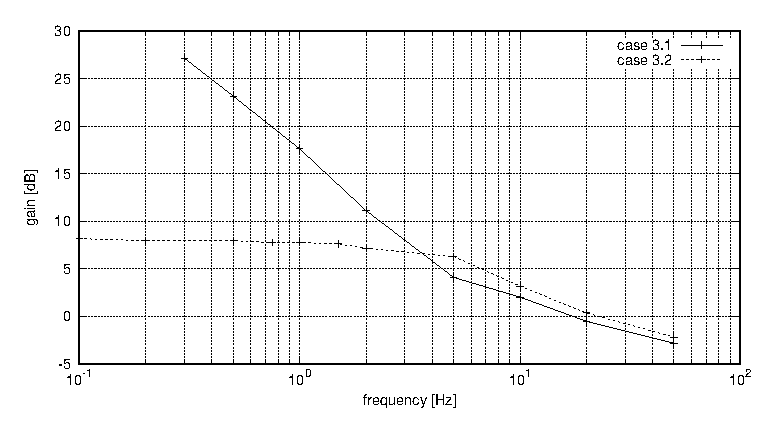
\includegraphics[keepaspectratio, scale=0.6]{../data/case3-g.eps}
    \subcaption{周波数対閉ループ利得特性}
  \end{minipage}
  \begin{minipage}{8cm}
    \centering
    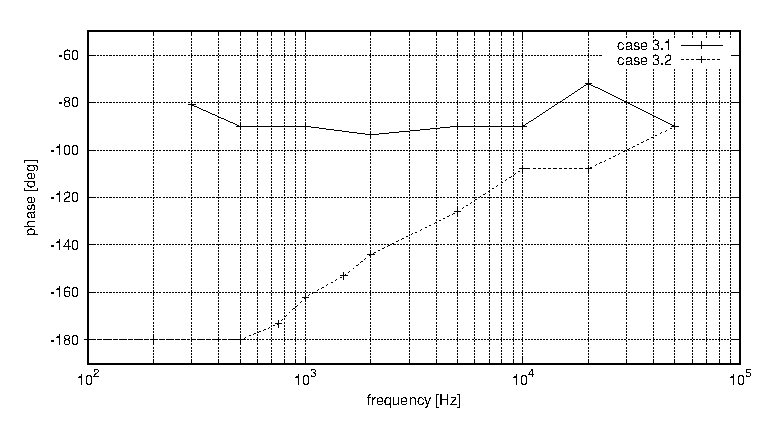
\includegraphics[keepaspectratio, scale=0.6]{../data/case3-f.eps}
    \subcaption{周波数対位相差特性}
  \end{minipage}
  \caption{case 3.1 3.2における回路特性測定結果}
  \label{fig:gr:case3}
\end{figure}

\subsection{case 4}
図\ref{fig:gr:case4}にcase 4の回路特性測定結果をグラフで示す.
\begin{figure}[H]
  \centering
  \begin{minipage}{8cm}
    \centering
    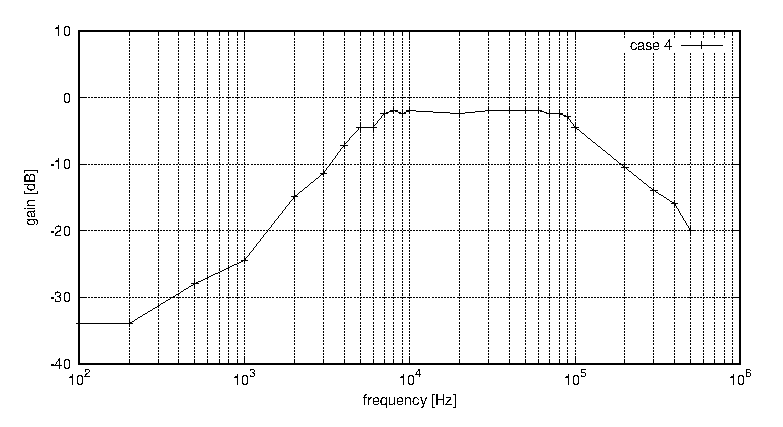
\includegraphics[keepaspectratio, scale=0.6]{../data/case4-g.eps}
    \subcaption{周波数対閉ループ利得特性}
  \end{minipage}
  \begin{minipage}{8cm}
    \centering
    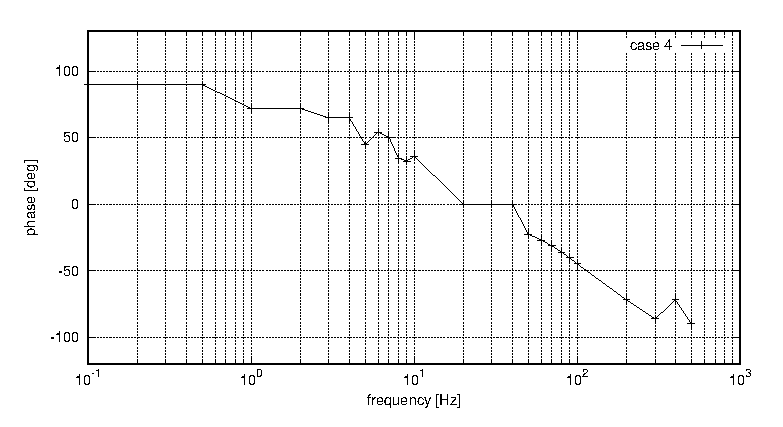
\includegraphics[keepaspectratio, scale=0.6]{../data/case4-f.eps}
    \subcaption{周波数対位相差特性}
  \end{minipage}
  \caption{case 4における回路特性測定結果}
  \label{fig:gr:case4}
\end{figure}


\begin{thebibliography}{99}
  \bibitem{ataka} 高橋 章、実験テキスト「信号処理プログラミング」、(2022年),
  \bibitem{ataka} 高橋 章、Wikipedia「標本化定理」、{https://ja.wikipedia.org/wiki/標本化定理} 、(2021年12月15日 (水) 12:16)
\end{thebibliography}

\end{document}